\documentclass{article}
\usepackage{graphicx}
\usepackage[dvipsnames]{xcolor}
\usepackage{tikz}
\usepackage{geometry}

\geometry{top=35mm, bottom=0mm, right=0mm, left=0mm}

\begin{document}
\thispagestyle{empty}

    \begin{center}

        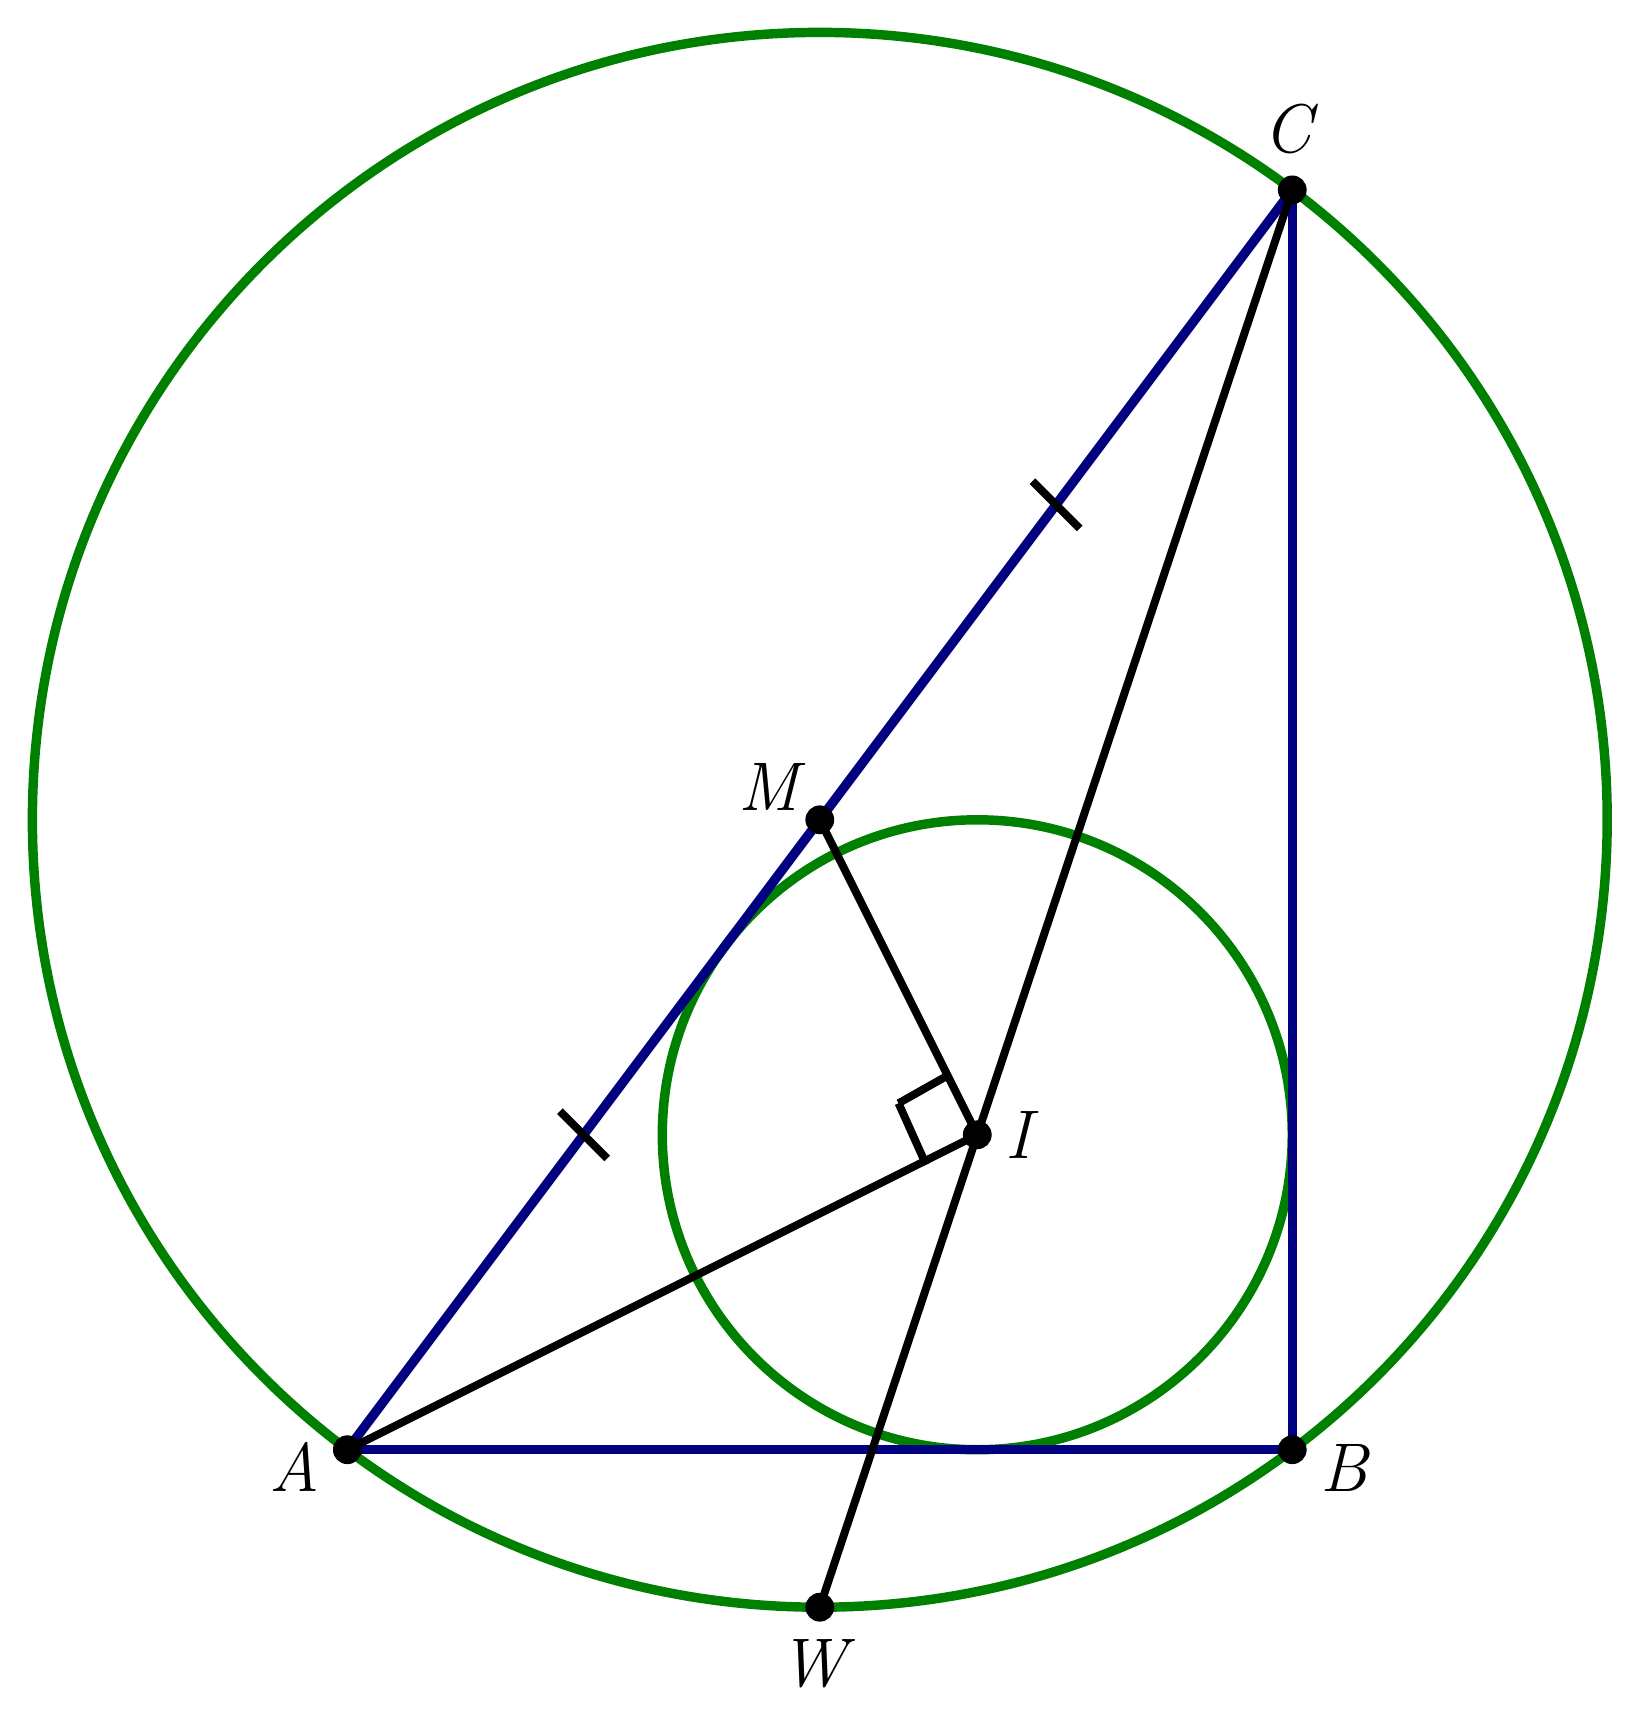
\begin{tikzpicture}

            \draw[Green, line width=1.2mm] (0,0) circle (10);

            \draw[Green, line width=1.2mm] (2,-4) circle (4);

            \draw[line width=1.2mm, NavyBlue] (6,8) -- (-6,-8);

            \draw[line width=1.2mm, NavyBlue] (-6,-8) -- (6,-8);

            \draw[line width=1.2mm, NavyBlue] (6,8) -- (6,-8);

            \draw[line width=1mm, Black] (6,8) -- (0,-10);

            \draw[line width=1mm, Black] (2,-4) -- (0,0);

            \draw[line width=1mm, Black] (2,-4) -- (-6,-8);

            \draw[line width=1mm, Black] (3,4) -- (2.7,4.3);
            \draw[line width=1mm, Black] (3,4) -- (3.3,3.7);

            \draw[line width=1mm, Black] (-3,-4) -- (-2.7,-4.3);
            \draw[line width=1mm, Black] (-3,-4) -- (-3.3,-3.7);

            \draw[line width=1mm, Black] (1,-3.6) -- (1.35,-4.38);
            \draw[line width=1mm, Black] (1,-3.6) -- (1.62,-3.25);

            \filldraw[black] (2,-4) circle (5pt);
            \node[right] at (2,-4) {{ } \Huge \textit I};

            \filldraw[black] (0,-10) circle (5pt);
            \node[below] at (0,-10) {\raisebox{-2.5em}{\Huge\textit{W}}};

            \filldraw[black] (6,8) circle (5pt);
            \node[above] at (6,8) {\raisebox{1em}{\Huge\textit{C}}};

            \filldraw[black] (-6,-8) circle (5pt);
            \node[left] at (-6,-8) {\raisebox{-3em}{\Huge\textit{A}} \raisebox{-3em}{ }};

            \filldraw[black] (6,-8) circle (5pt);
            \node[right] at (6,-8) {\raisebox{-3em}{ } \raisebox{-3em}{\Huge\textit{B}}};

            \filldraw[black] (0,0) circle (5pt);
            \node[above left] at (0,0) {\raisebox{0em}{ } \raisebox{0em}{\Huge\textit{M}}};

        \end{tikzpicture}
    
    \end{center}

\end{document}
